\chapter{Vremenska složenost}

\index{vremenska složenost}

Efikasnost algoritama važna je u natjecateljskom programiranju.
Obično je lako osmisliti algoritam
koji zadatak rješava sporo,
ali pravi je izazov osmisliti
brz algoritam.
Ako je algoritam prespor, dobit će samo
dio bodova ili neće dobiti nijedan bod.

\key{Vremenska složenost} algoritma
procjenjuje koliko će vremena algoritam utrošiti
za neki ulaz.
Ideja je prikazati efikasnost
kao funkciju čiji je parametar veličina ulaza.
Izračunavanjem vremenske složenosti
možemo utvrditi je li algoritam dovoljno brz
bez njegove implementacije.

\section{Pravila izračuna}

Vremenska složenost algoritma
označava se s $O(\cdots)$,
pri čemu tri točke predstavljaju neku
funkciju.
Varijabla $n$ obično označava
veličinu ulaza.
Primjerice, ako je ulaz niz brojeva,
$n$ će biti veličina niza,
a ako je ulaz znakovni niz,
$n$ će biti duljina znakovnog niza.

\subsubsection*{Petlje}

Čest razlog zbog kojeg je algoritam spor jest
to što sadrži mnogo petlji koje prolaze kroz ulaz.
Što algoritam sadrži više ugniježđenih petlji,
to je sporiji.
Ako postoji $k$ ugniježđenih petlji,
vremenska složenost iznosi $O(n^k)$.

Primjerice, vremenska složenost sljedećeg koda iznosi $O(n)$:
\begin{lstlisting}
for (int i = 1; i <= n; i++) {
    // code
}
\end{lstlisting}

A vremenska složenost sljedećeg koda iznosi $O(n^2)$:
\begin{lstlisting}
for (int i = 1; i <= n; i++) {
    for (int j = 1; j <= n; j++) {
        // code
    }
}
\end{lstlisting}

\subsubsection*{Red veličine}

Vremenska složenost ne govori nam točan broj
izvođenja koda unutar petlje,
nego prikazuje samo red veličine.
U sljedećim se primjerima kod unutar petlje
izvodi $3n$, $n+5$ i $\lceil n/2 \rceil$ puta,
ali vremenska složenost svakog koda iznosi $O(n)$.

\begin{lstlisting}
for (int i = 1; i <= 3*n; i++) {
    // code
}
\end{lstlisting}

\begin{lstlisting}
for (int i = 1; i <= n+5; i++) {
    // code
}
\end{lstlisting}

\begin{lstlisting}
for (int i = 1; i <= n; i += 2) {
    // code
}
\end{lstlisting}

Kao drugi primjer,
vremenska složenost sljedećeg koda iznosi $O(n^2)$:

\begin{lstlisting}
for (int i = 1; i <= n; i++) {
    for (int j = i+1; j <= n; j++) {
        // code
    }
}
\end{lstlisting}

\subsubsection*{Faze}

Ako se algoritam sastoji od uzastopnih faza,
ukupna vremenska složenost jednaka je najvećoj
vremenskoj složenosti pojedine faze.
Razlog je to što je najsporija
faza obično usko grlo koda.

Primjerice, sljedeći se kod sastoji
od triju faza s vremenskim složenostima
$O(n)$, $O(n^2)$ i $O(n)$.
Stoga ukupna vremenska složenost iznosi $O(n^2)$.

\begin{lstlisting}
for (int i = 1; i <= n; i++) {
    // code
}
for (int i = 1; i <= n; i++) {
    for (int j = 1; j <= n; j++) {
        // code
    }
}
for (int i = 1; i <= n; i++) {
    // code
}
\end{lstlisting}

\subsubsection*{Više varijabli}

Ponekad vremenska složenost ovisi o
više čimbenika.
U tom slučaju formula vremenske složenosti
sadrži više varijabli.

Primjerice, vremenska složenost
sljedećeg koda iznosi $O(nm)$:

\begin{lstlisting}
for (int i = 1; i <= n; i++) {
    for (int j = 1; j <= m; j++) {
        // code
    }
}
\end{lstlisting}

\subsubsection*{Rekurzija}

Vremenska složenost rekurzivne funkcije
ovisi o broju poziva funkcije
i vremenskoj složenosti pojedinog poziva.
Ukupna vremenska složenost jednaka je umnošku
tih vrijednosti.

Primjerice, razmotrimo sljedeću funkciju:
\begin{lstlisting}
void f(int n) {
    if (n == 1) return;
    f(n-1);
}
\end{lstlisting}
Poziv $\texttt{f}(n)$ uzrokuje $n$ poziva funkcije,
a vremenska složenost svakog poziva iznosi $O(1)$.
Stoga ukupna vremenska složenost iznosi $O(n)$.

Kao drugi primjer, razmotrimo sljedeću funkciju:
\begin{lstlisting}
void g(int n) {
    if (n == 1) return;
    g(n-1);
    g(n-1);
}
\end{lstlisting}
U ovom slučaju svaki poziv funkcije generira dva druga
poziva, osim za $n=1$.
Pogledajmo što se događa kada se $g$ pozove
s parametrom $n$.
Sljedeća tablica prikazuje pozive funkcije
koje proizvodi taj jedan poziv:
\begin{center}
\begin{tabular}{rr}
poziv funkcije & broj poziva \\
\hline
$g(n)$ & 1 \\
$g(n-1)$ & 2 \\
$g(n-2)$ & 4 \\
$\cdots$ & $\cdots$ \\
$g(1)$ & $2^{n-1}$ \\
\end{tabular}
\end{center}
Na temelju toga vremenska složenost iznosi
\[1+2+4+\cdots+2^{n-1} = 2^n-1 = O(2^n).\]

\section{Klase složenosti}

\index{klase složenosti}

Sljedeća lista sadrži uobičajene vremenske složenosti
algoritama:

\begin{description}
\item[$O(1)$]
\index{algoritam konstantnog vremena}
Vrijeme izvođenja \key{algoritma konstantnog vremena}
ne ovisi o veličini ulaza.
Tipičan algoritam konstantnog vremena izravna je
formula koja izračunava odgovor.

\item[$O(\log n)$]
\index{logaritamski algoritam}
\key{Logaritamski} algoritam često prepolovi
veličinu ulaza u svakom koraku.
Vrijeme izvođenja takvog algoritma
logaritamsko je jer je
$\log_2 n$ jednak broju dijeljenja
broja $n$ s 2 potrebnih da se dobije 1.

\item[$O(\sqrt n)$]
\key{Algoritam kvadratnog korijena} sporiji je od
$O(\log n)$, ali brži od $O(n)$.
Posebno je svojstvo kvadratnih korijena da vrijedi
$\sqrt n = n/\sqrt n$, pa se kvadratni korijen $\sqrt n$ nalazi,
u određenom smislu, u sredini ulaza.

\item[$O(n)$]
\index{linearni algoritam}
\key{Linearni} algoritam prolazi kroz ulaz
konstantan broj puta.
To je često najbolja moguća vremenska složenost
jer je obično svakom
elementu ulaza potrebno pristupiti barem jednom prije
ispisivanja odgovora.

\item[$O(n \log n)$]
Ova vremenska složenost često pokazuje da
algoritam sortira ulaz
jer vremenska složenost efikasnih
algoritama za sortiranje iznosi $O(n \log n)$.
Druga je mogućnost da algoritam
koristi strukturu podataka u kojoj svaka operacija
traje $O(\log n)$ vremena.

\item[$O(n^2)$]
\index{kvadratni algoritam}
\key{Kvadratni} algoritam često sadrži
dvije ugniježđene petlje.
Kroz sve parove elemenata
ulaza moguće je proći u $O(n^2)$ vremenu.

\item[$O(n^3)$]
\index{kubni algoritam}
\key{Kubni} algoritam često sadrži
tri ugniježđene petlje.
Kroz sve trojke elemenata
ulaza moguće je proći u $O(n^3)$ vremenu.

\item[$O(2^n)$]
Ova vremenska složenost često pokazuje da
algoritam prolazi kroz sve
podskupove elemenata ulaza.
Primjerice, podskupovi skupa $\{1,2,3\}$ jesu
$\emptyset$, $\{1\}$, $\{2\}$, $\{3\}$, $\{1,2\}$,
$\{1,3\}$, $\{2,3\}$ i $\{1,2,3\}$.

\item[$O(n!)$]
Ova vremenska složenost često pokazuje da
algoritam prolazi kroz sve
permutacije elemenata ulaza.
Primjerice, permutacije skupa $\{1,2,3\}$ jesu
$(1,2,3)$, $(1,3,2)$, $(2,1,3)$, $(2,3,1)$,
$(3,1,2)$ i $(3,2,1)$.

\end{description}

\index{polinomni algoritam}
Algoritam je \key{polinomni}
ako je njegova vremenska složenost najviše $O(n^k)$,
pri čemu je $k$ konstanta.
Sve prethodno navedene vremenske složenosti osim
$O(2^n)$ i $O(n!)$ polinomne su.
U praksi je konstanta $k$ obično mala
pa polinomna vremenska složenost
ugrubo znači da je algoritam \emph{efikasan}.

\index{NP-težak zadatak}

Većina algoritama u ovoj knjizi polinomna je.
Ipak, postoje mnogi važni zadaci za koje
nije poznat nijedan polinomni algoritam, tj.
nitko ih ne zna efikasno riješiti.
\key{NP-teški} zadaci važan su skup
zadataka za koje nijedan polinomni algoritam
nije poznat\footnote{Klasična knjiga o toj temi djelo je
M. R. Gareyja i D. S. Johnsona
\emph{Računala i nerješivost: Vodič kroz teoriju
NP-potpunosti} \cite{gar79}.}.

\section{Procjena efikasnosti}

Izračunavanjem vremenske složenosti algoritma
možemo prije njegove
implementacije provjeriti je li
dovoljno efikasan za zadatak.
Polazište procjena jest činjenica da
moderno računalo može izvesti nekoliko stotina
milijuna operacija u sekundi.

Primjerice, pretpostavimo da je vremensko ograničenje
zadatka jedna sekunda, a veličina ulaza $n=10^5$.
Ako je vremenska složenost $O(n^2)$,
algoritam će izvesti oko $(10^5)^2=10^{10}$ operacija.
To bi trebalo trajati barem nekoliko desetaka sekundi
pa se čini da je algoritam prespor za rješavanje zadatka.

S druge strane, iz zadane veličine ulaza
možemo pokušati \emph{pogoditi}
potrebnu vremensku složenost algoritma
koji rješava zadatak.
Sljedeća tablica sadrži nekoliko korisnih procjena
uz pretpostavljeno vremensko ograničenje od jedne sekunde.

\begin{center}
\begin{tabular}{ll}
veličina ulaza & potrebna vremenska složenost \\
\hline
$n \le 10$ & $O(n!)$ \\
$n \le 20$ & $O(2^n)$ \\
$n \le 500$ & $O(n^3)$ \\
$n \le 5000$ & $O(n^2)$ \\
$n \le 10^6$ & $O(n \log n)$ ili $O(n)$ \\
$n$ je velik & $O(1)$ ili $O(\log n)$ \\
\end{tabular}
\end{center}

Primjerice, ako je veličina ulaza $n=10^5$,
vjerojatno se očekuje da vremenska
složenost algoritma iznosi $O(n)$ ili $O(n \log n)$.
Ta nam informacija olakšava osmišljavanje algoritma
jer isključuje pristupe koji bi dali
algoritam s većom vremenskom složenošću.

\index{konstantni faktor}

Ipak, važno je zapamtiti da je
vremenska složenost samo procjena efikasnosti
jer skriva \emph{konstantne faktore}.
Primjerice, algoritam koji se izvodi u $O(n)$ vremenu
može izvesti $n/2$ ili $5n$ operacija.
To znatno utječe na stvarno
vrijeme izvođenja algoritma.

\section{Najveća suma podniza}

\index{najveća suma podniza}

Često postoji više mogućih algoritama
za rješavanje zadatka čije se
vremenske složenosti razlikuju.
U ovom odjeljku razmatramo klasičan zadatak koji
ima izravno $O(n^3)$ rješenje.
Međutim, osmišljavanjem boljeg algoritma
zadatak je moguće riješiti u $O(n^2)$
vremenu, pa čak i u $O(n)$ vremenu.

Za zadani niz od $n$ brojeva,
naš je zadatak izračunati
\key{najveću sumu podniza}, tj.
najveću moguću sumu
niza uzastopnih vrijednosti
u nizu\footnote{Knjiga J. Bentleyja
\emph{Programmerski biseri} \cite{ben86} popularizirala je taj zadatak.}.
Zadatak je zanimljiv kada se u nizu mogu nalaziti
negativne vrijednosti.
Primjerice, u nizu
\begin{center}
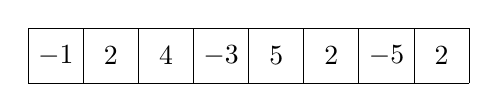
\begin{tikzpicture}[scale=0.7]
\draw (0,0) grid (8,1);

\node at (0.5,0.5) {$-1$};
\node at (1.5,0.5) {$2$};
\node at (2.5,0.5) {$4$};
\node at (3.5,0.5) {$-3$};
\node at (4.5,0.5) {$5$};
\node at (5.5,0.5) {$2$};
\node at (6.5,0.5) {$-5$};
\node at (7.5,0.5) {$2$};
\end{tikzpicture}
\end{center}
\begin{samepage}
sljedeći podniz daje najveću sumu $10$:
\begin{center}
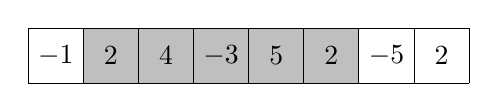
\begin{tikzpicture}[scale=0.7]
\fill[color=lightgray] (1,0) rectangle (6,1);
\draw (0,0) grid (8,1);

\node at (0.5,0.5) {$-1$};
\node at (1.5,0.5) {$2$};
\node at (2.5,0.5) {$4$};
\node at (3.5,0.5) {$-3$};
\node at (4.5,0.5) {$5$};
\node at (5.5,0.5) {$2$};
\node at (6.5,0.5) {$-5$};
\node at (7.5,0.5) {$2$};
\end{tikzpicture}
\end{center}
\end{samepage}

Pretpostavljamo da je prazan podniz dopušten
pa je najveća suma podniza uvijek barem $0$.

\subsubsection{Algoritam 1}

Izravan način rješavanja zadatka
jest proći kroz sve moguće podnizove,
izračunati sumu vrijednosti u svakom podnizu i pamtiti
najveću sumu.
Sljedeći kod implementira taj algoritam:

\begin{lstlisting}
int best = 0;
for (int a = 0; a < n; a++) {
    for (int b = a; b < n; b++) {
        int sum = 0;
        for (int k = a; k <= b; k++) {
            sum += array[k];
        }
        best = max(best,sum);
    }
}
cout << best << "\n";
\end{lstlisting}

Varijable \texttt{a} i \texttt{b} određuju prvi i
posljednji indeks podniza,
a suma vrijednosti izračunava se u varijablu \texttt{sum}.
Varijabla \texttt{best} sadrži najveću sumu pronađenu tijekom pretraživanja.

Vremenska složenost algoritma iznosi $O(n^3)$
jer se sastoji od triju ugniježđenih petlji
koje prolaze kroz ulaz.

\subsubsection{Algoritam 2}

Algoritam 1 lako je učiniti efikasnijim
uklanjanjem jedne petlje.
To je moguće učiniti izračunavanjem sume u isto
vrijeme kada se pomiče desni kraj podniza.
Rezultat je sljedeći kod:

\begin{lstlisting}
int best = 0;
for (int a = 0; a < n; a++) {
    int sum = 0;
    for (int b = a; b < n; b++) {
        sum += array[b];
        best = max(best,sum);
    }
}
cout << best << "\n";
\end{lstlisting}
Nakon ove promjene vremenska složenost iznosi $O(n^2)$.

\subsubsection{Algoritam 3}

Iznenađujuće, zadatak je moguće riješiti
u $O(n)$ vremenu\footnote{U \cite{ben86} ovaj se algoritam linearnog vremena
pripisuje J. B. Kadaneu, a algoritam se ponekad
naziva \index{Kadaneov algoritam} \key{Kadaneov algoritam}.}, što znači
da je dovoljna samo jedna petlja.
Ideja je za svaki položaj u nizu izračunati
najveću sumu podniza koji završava na tom položaju.
Nakon toga rješenje zadatka predstavlja
najveća od tih suma.

Razmotrimo podzadatak pronalaženja podniza najveće sume
koji završava na položaju $k$.
Postoje dvije mogućnosti:
\begin{enumerate}
\item Podniz sadrži samo element na položaju $k$.
\item Podniz se sastoji od podniza koji završava
na položaju $k-1$, nakon kojeg slijedi element na položaju $k$.
\end{enumerate}

U drugom slučaju, budući da želimo
pronaći podniz najveće sume,
podniz koji završava na položaju $k-1$
također treba imati najveću sumu.
Stoga zadatak možemo efikasno riješiti
izračunavanjem najveće sume podniza
za svaki završni položaj slijeva nadesno.

Sljedeći kod implementira algoritam:
\begin{lstlisting}
int best = 0, sum = 0;
for (int k = 0; k < n; k++) {
    sum = max(array[k],sum+array[k]);
    best = max(best,sum);
}
cout << best << "\n";
\end{lstlisting}

Algoritam sadrži samo jednu petlju
koja prolazi kroz ulaz
pa vremenska složenost iznosi $O(n)$.
To je ujedno najbolja moguća vremenska složenost
jer svaki algoritam za ovaj zadatak
mora barem jednom pregledati sve elemente niza.

\subsubsection{Usporedba efikasnosti}

Zanimljivo je proučiti koliko su algoritmi
efikasni u praksi.
Sljedeća tablica prikazuje vremena izvođenja
prethodno navedenih algoritama za različite
vrijednosti $n$ na modernom računalu.

U svakom je testu ulaz generiran nasumično.
Vrijeme potrebno za čitanje ulaza nije
izmjereno.

\begin{center}
\begin{tabular}{rrrr}
veličina niza $n$ & Algoritam 1 & Algoritam 2 & Algoritam 3 \\
\hline
$10^2$ & $0.0$ s & $0.0$ s & $0.0$ s \\
$10^3$ & $0.1$ s & $0.0$ s & $0.0$ s \\
$10^4$ & > $10.0$ s & $0.1$ s & $0.0$ s \\
$10^5$ & > $10.0$ s & $5.3$ s & $0.0$ s \\
$10^6$ & > $10.0$ s & > $10.0$ s & $0.0$ s \\
$10^7$ & > $10.0$ s & > $10.0$ s & $0.0$ s \\
\end{tabular}
\end{center}

Usporedba pokazuje da su svi algoritmi
efikasni kada je veličina ulaza mala,
ali veći ulazi otkrivaju znatne
razlike u vremenima izvođenja algoritama.
Algoritam 1 postaje spor
kada je $n=10^4$, a Algoritam 2
postaje spor kada je $n=10^5$.
Samo Algoritam 3 može trenutačno obraditi
čak i najveće ulaze.
